\documentclass{standalone}
\usepackage{tikz}
\usepackage{ctex,siunitx}
\usepackage{tkz-euclide}
\usepackage{amsmath}
\usetikzlibrary{patterns, calc}
\usetikzlibrary {decorations.pathmorphing, decorations.pathreplacing, decorations.shapes,}
\begin{document}
\small
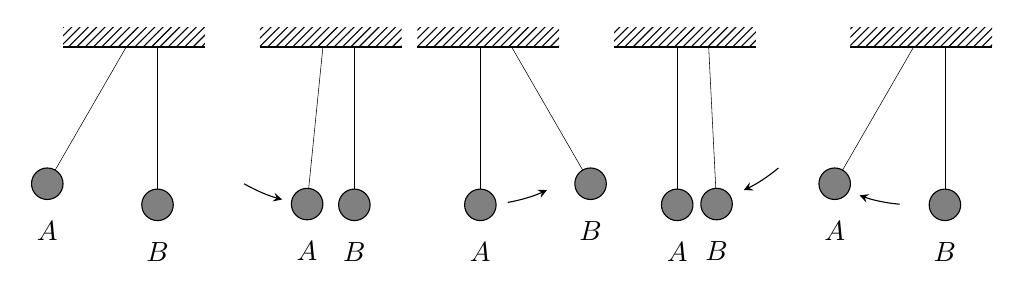
\begin{tikzpicture}[>=stealth, scale=1]
  \begin{scope}
  \fill[pattern=north east lines](-0.8,0) rectangle (1,.25);
  \draw[thick](-0.8,0)--(1,0);
  \tkzDefPoints{0/0/A', 0.4/0/B', 0.4/-2/B, -1/-1.732/A}
  \tkzDrawSegments(A,A' B,B')
  \draw[fill=gray](A) circle(.2);
  \draw[fill=gray](B) circle(.2);
  \tkzLabelPoints[below=10pt](A,B)
  \end{scope}
  \begin{scope}[xshift=2.5cm]
      \fill[pattern=north east lines](-0.8,0) rectangle (1,.25);
      \draw[thick](-0.8,0)--(1,0);
  \tkzDefPoints{0/0/A', 0.4/0/B', 0.4/-2/B, -.2/-1.99/A}
  \tkzDrawSegments(A,A' B,B')
  \draw[fill=gray](A) circle(.2);
  \draw[fill=gray](B) circle(.2);
  \tkzLabelPoints[below=10pt](A,B)
  \draw[->](-120:2) arc (-120:-105:2);
  \end{scope}
  \begin{scope}[xshift=4.5cm]
      \fill[pattern=north east lines](-0.8,0) rectangle (1,.25);
      \draw[thick](-0.8,0)--(1,0);
  \tkzDefPoints{0/0/A', 0.4/0/B', 0/-2/A, 1.4/-1.732/B}
  \tkzDrawSegments(A,A' B,B')
  \draw[fill=gray](A) circle(.2);
  \draw[fill=gray](B) circle(.2);
  \tkzLabelPoints[below=10pt](A,B)
  \draw[->](-80:2) arc (-80:-65:2);
  \end{scope}
  \begin{scope}[xshift=7cm]
      \fill[pattern=north east lines](-0.8,0) rectangle (1,.25);
      \draw[thick](-0.8,0)--(1,0);
  \tkzDefPoints{0/0/A', 0.4/0/B', 0.5/-1.99/B, 0/-2/A}
  \tkzDrawSegments(A,A' B,B')
  \draw[fill=gray](A) circle(.2);
  \draw[fill=gray](B) circle(.2);
  \tkzLabelPoints[below=10pt](A,B)
  \draw[<-](-65:2) arc (-65:-50:2);
  \end{scope}
  \begin{scope}[xshift=10cm]
      \fill[pattern=north east lines](-0.8,0) rectangle (1,.25);
      \draw[thick](-0.8,0)--(1,0);
  \tkzDefPoints{0/0/A', 0.4/0/B', 0.4/-2/B, -1/-1.732/A}
  \tkzDrawSegments(A,A' B,B')
  \draw[fill=gray](A) circle(.2);
  \draw[fill=gray](B) circle(.2);
  \tkzLabelPoints[below=10pt](A,B)
  \draw[<-](-110:2) arc (-110:-95:2);
  \end{scope}
\end{tikzpicture}
\end{document}